
\begin{exo}
  \donnee{La fonction de répartition d’une variable aléatoire X est}
  \[ F_\text{x}(x)= \begin{cases} 
    0   &\text{ si } x< 5 \\
    0.2 &\text{ si } 5\leq x< 7 \\
    0.3 &\text{ si } 7\leq x< 8 \\
    0.7 &\text{ si } 8\leq x< 10 \\
    0.8 &\text{ si } 10\leq x< 11 \\
    1   &\text{ si } x \ge 11 \\
 \end{cases}\]
 \begin{subexo}{Représenter garaphiquement la fonction de répartition de $X$}
  \begin{center}
    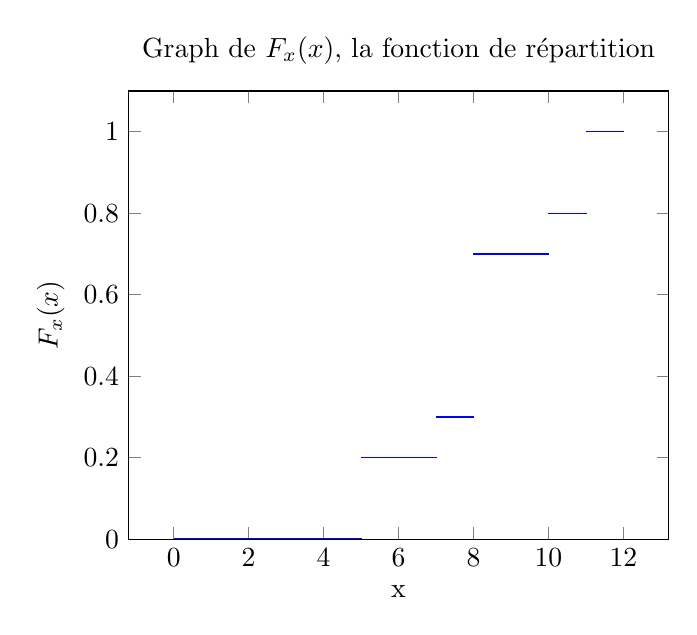
\begin{tikzpicture}[]
      \begin{axis}[
        ymin=0,
        domain=0:15,
        samples=400,
        xlabel={x},
        ylabel={$F_\text{x}(x)$},
        title={Graph de $F_\text{x}(x)$, la fonction de répartition},
      ]
        \addplot [color=blue,domain=0:5] {0.001};
        \addplot [color=blue,domain=5:7] {0.2};
        \addplot [color=blue,domain=7:8] {0.3};
        \addplot [color=blue,domain=8:10] {0.7};
        \addplot [color=blue,domain=10:11] {0.8};
        \addplot [color=blue,domain=11:12] {1};


      \end{axis}
    \end{tikzpicture} 
  \end{center}
 \end{subexo}
  \begin{subexo}{Déterminer les réalisations de la variable aléatoire $X$ ainsi que sa loi de probabilité}
    Pour rappel nous avons \begin{equation}F_\text{x}(x) =  P(X \le x)\end{equation}.
    Autrement dit nous avons $$F_\text{x}(x) = \sum_{x_i \le x}{P(X = x_i)}$$
    Faisons un exemple avec $x = 7$
    \begin{align*} F_x(7) &= \sum_{x_i \le 7}{P(X = x_i)} \\
      &= P(X = 5) + P(X=7) \\
        P(X=7) &= F_x(7) - P(X=5)\\
        &= 0.3 - 0.2 \\
        &= 0.1 
      \end{align*}
    \begin{center}
      \begin{tabular}{@{}l|lllll@{}}
        \toprule
        $X = x$  & 5   & 7   & 8   & 10  & 11  \\ \midrule
        $P(X=x)$ & 0.2 & 0.1 & 0.4 & 0.1 & 0.2 \\ \bottomrule
        \end{tabular}
    \end{center}
  \end{subexo}
  \begin{subexo}{Calculer les probabilité $P(X \le 6.5)$, $P(8 < X \le 10)$,$P( 8 \le X \le 10 )$,$P(X >10)$,}
    Nous avons $F_x(X \le 6.5) $ puisque (1) et donc 
    \begin{align*}
      F_x(X \le 6.5)  &= \underbrace{P(X \le 5)}_0 + \underbrace{P( 5 < X \le 6.5)}_{0.2}\\
       &=0.2 
    \end{align*}
  \end{subexo}
  \begin{subexo}{Sans calcul, déterminer l'espérance de $X$}
    Par définition l'espérance $$\mathbb{E}(X) \text{ est égal à } \sum_{i=1}^{n} x_i \cdot P(X=x_i)$$\newline
Mais on peut la trouver  facilement en reprenant la lois de probabilité de b), en effet on peut voir que les valeur sont symétrique autour de 8, avec les mêmes probabilités
Donc on aura la moyenne pondérée égale à 8
\end{subexo}
\end{exo}
